While the simulations involve purely DV$\pi^0$P events, the raw experimental data is a combination of all reactions possible at the designated kinematics. To be classified as a DV$\pi^0$P event there are a number of criteria, called exclusivity cuts, that must be satisfied. It is helpful to first define the relevant variables:


\begin{align}
IM^{2}_{\pi^{0}} &= p^{2}_{\pi^{0}} = (p_{\gamma1} + p_{\gamma2})^{2}  \\
ME_{e'p'\pi^{0}} &= E_{beam} + M - E_{e'} - E_{p'} - E_{\gamma1}E_{\gamma2} \\
MM^{2}_{e'p'\pi^{0}} &= (p_{beam} + p_{target} - p_{e'} - p_{p'} - p_{\gamma1} - p_{\gamma2})^{2}  \\
MM^{2}_{e'p'} &= (p_{beam} + p_{target} - p_{e'} - p_{p'})^{2} \\
MM^{2}_{e'\pi^{0}} &= (p_{beam} + p_{target} - p_{e'} - p_{\gamma1} - p_{\gamma2})^{2} \\
MP_{te'p'\gamma} &= \sqrt{(p_{beam} + p_{target} - p_{e'} - p_{\gamma1} - p_{\gamma2})^{2}_{x} + (p_{beam} + p_{target} - p_{e'} - p_{\gamma1} - p_{\gamma2})^{2}_{y}}\\
\theta_{\pi^{0}_{det.\pi^{0}_{rec.}}} &= \angle(p_{\gamma1} + p_{\gamma2} , p_{beam} + p_{target} - p_{e'} - p_{p'}) \\
\phi_{H\Pi} &= \angle(\vec{H}, \vec{\delta})
\end{align}

For a DV$\pi^0$P event measured in a perfect-resolution system, we would have:
\begin{itemize}
    \item $IM^{2}_{\pi^{0}}$ = $\pi^0$ mass = 134.976 MeV/c 
    \item $ME_{e'p'\pi^{0}}$ = 0 
    \item $MM^{2}_{e'p'\pi^{0}}$ = 0 
    \item $MM^{2}_{e'p'}$ = 0 
    \item $MP_{te'p'\pi^{0}}$ = 0 
    \item $\theta_{\pi^{0}_{det.\pi^{0}_{rec.}}}$ = 0 
    \item $\phi_{H\Pi}$ = 0 
    \item $MM^{2}_{e'\gamma} = m^{2}_{p}$.
\end{itemize}


In reality, detector resolutions and reconstruction schemes are of course imperfect, and so no real event will satisfy the criteria above. Instead, we define cut values to decide which events are close enough to be considered a signal event.  For this analysis, we chose a standard 3$\sigma$ cut on variable distributions to define exclusive events. 


    The relevant 1D exclusive distributions are shown on the Fig.~\ref{fig:rawexclusive1} and \ref{fig:rawexclusive2}.
    
    \begin{figure}[hbt]
    	\centering
    	\includegraphics[page=4,width=0.47\linewidth]{Chapters/Ch4-BaseAnalysis/1_Event_Selection_Cuts/figures/eppi0.exclusive.pdf}
    	\includegraphics[page=5,width=0.47\linewidth]{Chapters/Ch4-BaseAnalysis/1_Event_Selection_Cuts/figures/eppi0.exclusive.pdf}
    	\caption{Event distributions for events with at least one electron, proton and two photons.}
    	\label{fig:rawexclusive1}
    \end{figure}
    
    \begin{figure}[hbt]
    	\centering
    	\includegraphics[page=6,width=0.47\linewidth]{Chapters/Ch4-BaseAnalysis/1_Event_Selection_Cuts/figures/eppi0.exclusive.pdf}
    	\includegraphics[page=8,width=0.47\linewidth]{Chapters/Ch4-BaseAnalysis/1_Event_Selection_Cuts/figures/eppi0.exclusive.pdf}
    	\caption{Event distributions for events with at least one electron, proton and two photons.}
    	\label{fig:rawexclusive2}
    \end{figure}
    
    \subsubsection{Tight \texorpdfstring{$M_{\gamma\gamma} $} mass and transverse missing momenta cuts}
    
    The first step is to use tighter $\gamma\gamma$ mass cut: $0.096<M_{\gamma\gamma}<0.168$ GeV, and take a look at the missing transverse momentum distributions (see Fig.~\ref{fig:ptdistributions}).
    From momentum conservation law we expect transverse momentum to be zero, so we can apply cuts on $\Delta p_x$ and $\Delta p_y$ to further improve exclusive channel selection.
    The cuts $|\Delta p_x|<0.2$ and $|\Delta p_y|<0.2$ correspond roughly to 4-5 $\sigma$.
    
    \begin{figure}[hbt]
    	\centering
    	\includegraphics[page=24,width=0.47\linewidth]{Chapters/Ch4-BaseAnalysis/1_Event_Selection_Cuts/figures/eppi0.exclusive.pdf}
    	\includegraphics[page=25,width=0.47\linewidth]{Chapters/Ch4-BaseAnalysis/1_Event_Selection_Cuts/figures/eppi0.exclusive.pdf}
    	\caption{Exclusive distributions for events with at least one electron, proton and two photons.}
    	\label{fig:ptdistributions}
    \end{figure}
    
    The exclusive distributions after tight $M_{\gamma\gamma}$ mass and transverse missing momenta cuts are shown on Fig.~\ref{fig:rawexclusive3} and display much stronger signal peaks on top of reduced background.
    
    \begin{figure}[hbt]
    	\centering
    	\includegraphics[page=43,width=0.45\linewidth]{Chapters/Ch4-BaseAnalysis/1_Event_Selection_Cuts/figures/eppi0.exclusive.pdf}
    	\includegraphics[page=44,width=0.45\linewidth]{Chapters/Ch4-BaseAnalysis/1_Event_Selection_Cuts/figures/eppi0.exclusive.pdf}
    	\includegraphics[page=45,width=0.45\linewidth]{Chapters/Ch4-BaseAnalysis/1_Event_Selection_Cuts/figures/eppi0.exclusive.pdf}
        \includegraphics[page=47,width=0.45\linewidth]{Chapters/Ch4-BaseAnalysis/1_Event_Selection_Cuts/figures/eppi0.exclusive.pdf}
    
    	\caption{Exclusive distributions after tight $M_{\gamma\gamma}$ mass and transverse missing momenta cuts .}
    	\label{fig:rawexclusive3}
    \end{figure}
    


    The complete list of event cuts, including fiducial (chapter 2), DIS, and exclusivity cuts are:

   \iffalse
    \begin{itemize}
    \item at least one electron, one proton, two photon in the final state.
    \item $E_{p'} > 0.94358$ GeV
    \item $\theta_{e'\gamma1}$, $\theta_{e'\gamma2} > 4^{\circ}$
    \item $E_{\gamma1}$, $E_{\gamma2} > 0.15$ GeV
    \item $\theta_{\gamma1\gamma2} > 1^{\circ}$
    \item $-1.5$ GeV $< ME_{e'p'\pi^{0}} < 2$ GeV
    \item $0$ GeV $< ME_{e'\gamma} < 2.5$ GeV
    \item $|MM^{2}_{e'p'\pi^{0}}| < 0.1$ GeV$^{2}$
    \item $MP^{2}_{te'p'\gamma} < 0.75$ GeV$^{2}$
    \end{itemize}
    \fi


    \begin{itemize}
    \item $p_{e'} > 2 \, \text{GeV/c}$
    \item $p_{\gamma} > 2 \, \text{GeV/c} \, (\text{BH-DVCS}), \, p_{\gamma}^{2} > 0.4 \, \text{GeV/c} \, (\text{DV}\pi^{0}\text{P})$
    \item $p_{p'} > 0.3 \, \text{GeV/c} \, (\text{CD}), \, 0.42 \, \text{GeV/c} \, (\text{FD, Inb.}), \, 0.5 \, \text{GeV/c} \, (\text{FD, Outb.})$
    \item $Q^{2} > 1 \, (\text{GeV/c})^{2}$
    \item $W > 2 \, \text{GeV}$
    \item Electron not in same sector as photons. 
    \item The protons reconstructed in the same sector with photons were excluded when the protons have associated hits in the FD ECAL.
    \item $E_{p'} > 0.94358$ GeV
    \item $\theta_{e'\gamma1}$, $\theta_{e'\gamma2} > 4^{\circ}$
    \item $E_{\gamma1}$, $E_{\gamma2} > 0.15$ GeV
    \item $\theta_{\gamma1\gamma2} > 1^{\circ}$
    \item $-1.5$ GeV $< ME_{e'p'\pi^{0}} < 2$ GeV
    \item $0$ GeV $< ME_{e'\gamma} < 2.5$ GeV
    \item $|MM^{2}_{e'p'\pi^{0}}| < 0.1$ GeV$^{2}$
    \item $MP^{2}_{te'p'\gamma} < 0.75$ GeV$^{2}$
    
    \iffalse
    \item The $3\sigma$ exclusivity cuts described in this section were applied.
    
    \item $lb_{IM\pi^{0}} < IM\pi^{0} < ub_{IM\pi^{0}}$
    \item $lb_{MM^{2}_{e'p'}} < MM^{2}_{e'p'} < ub_{MM^{2}_{e'p'}}$
    \item $lb_{MM^{2}_{e'\pi^{0}}} < MM^{2}_{e'\pi^{0}} < ub_{MM^{2}_{e'\pi^{0}}}$
    \item $lb_{MM^{2}_{e'p'\pi^{0}}} < MM^{2}_{e'p'\pi^{0}} < ub_{MM^{2}_{e'p'\pi^{0}}}$
    \item $lb_{ME_{e'p'\pi^{0}}} < ME_{e'p'\pi^{0}} < ub_{ME_{e'p'\pi^{0}}}$
    \item $lb_{MPt_{e'p'\pi^{0}}} < MPt_{e'p'\pi^{0}} < ub_{MPt_{e'p'\pi^{0}}}$
    \item $\theta_{\pi^{0}_{det.\pi^{0}_{rec.}}} < ub_{\theta_{\pi^{0}_{det.\pi^{0}_{rec.}}}}$
    \fi
    \end{itemize}


    Each event was tested against this set of criteria. For events with more than two photons, every permutation of two photons was tested, and the event was classified as a signal event if at least one combination passed all cuts. If more than combination passed cuts, the two photons with the invariant photon-photon mass closest to the neutral pion mass was selected. Exclusive distributions after all exclusivity cuts except $MM^2(epX)<0.5$ GeV are shown on Fig.~\ref{fig:finalexclusive}
    
    \begin{figure}[hbt]
    	\centering
    	
    	\includegraphics[page=82,width=0.32\linewidth]{Chapters/Ch4-BaseAnalysis/1_Event_Selection_Cuts/figures/eppi0.exclusive.pdf}
    	\includegraphics[page=83,width=0.32\linewidth]{Chapters/Ch4-BaseAnalysis/1_Event_Selection_Cuts/figures/eppi0.exclusive.pdf}
    	\includegraphics[page=84,width=0.32\linewidth]{Chapters/Ch4-BaseAnalysis/1_Event_Selection_Cuts/figures/eppi0.exclusive.pdf}
    	\caption{Exclusive distributions after all exclusivity cuts .}
    	\label{fig:finalexclusive}
    \end{figure}











\iffalse



    \begin{figure}
        \centering
       \includegraphics[page=10,width=0.97\linewidth]{Chapters/Ch4-BaseAnalysis/1_Event_Selection_Cuts/figures/eppi0.exclusive.pdf}
    	\caption{MM$^2$ (epX) vs $\theta_X\pi$ 2D distribution.}
    	\label{fig:MM2vsThetaXPi}
    \end{figure}


   

    \subsubsection{\texorpdfstring{$\theta_{X\pi}$} cut determination}
    
    The cut on angle between expected and reconstructed pion is used in order to further reduce background.
    To choose the value of the $\theta_{X\pi}$ cut the $MM^2(epX)$ distribution is analyzed at multiple $\theta_{X\pi}$ cut values and fit using gaussian+polynomial function as shown on Fig.~\ref{fig:mm2fordifferenttheta}.
    From the fit we can estimate the number of good exclusive events (gaussian) and the number of background events (polynomial) and their dependence on $\theta_{X\pi}$ cut.
    Fig.~\ref{fig:sigbgvsthetacutQ2} and~\ref{fig:sigbgvsthetacutxB} show the numbers of signal and background events as functions of $\theta_{X\pi}$ cut value for multiple bins in $Q^2$ and $x_B$.
    These plots show that the cut $\theta_{X\pi}<2^\circ$ allows to select the most number of good events with the least background, and relaxing it beyond $2^\circ$ does not gain us any good exclusive events but increases background.
    
    
    \begin{figure}[hbt]
    	\centering
    	\includegraphics[page=123,width=0.3\linewidth]{Chapters/Ch4-BaseAnalysis/1_Event_Selection_Cuts/figures/sigbg_eppi0.pdf}
    	\includegraphics[page=125,width=0.3\linewidth]{Chapters/Ch4-BaseAnalysis/1_Event_Selection_Cuts/figures/sigbg_eppi0.pdf}
    	\includegraphics[page=128,width=0.3\linewidth]{Chapters/Ch4-BaseAnalysis/1_Event_Selection_Cuts/figures/sigbg_eppi0.pdf}
    	\includegraphics[page=130,width=0.3\linewidth]{Chapters/Ch4-BaseAnalysis/1_Event_Selection_Cuts/figures/sigbg_eppi0.pdf}
    	\includegraphics[page=133,width=0.3\linewidth]{Chapters/Ch4-BaseAnalysis/1_Event_Selection_Cuts/figures/sigbg_eppi0.pdf}
    	\includegraphics[page=135,width=0.3\linewidth]{Chapters/Ch4-BaseAnalysis/1_Event_Selection_Cuts/figures/sigbg_eppi0.pdf}
    	
    	\caption{$MM^2(epX)$ distributions for multiple $\theta_{X\pi}$ cut values.}
    	\label{fig:mm2fordifferenttheta}
    \end{figure}
    
    
    \begin{figure}[hbt]
    	\centering
    	
    	\includegraphics[width=0.32\linewidth,page=34]{Chapters/Ch4-BaseAnalysis/1_Event_Selection_Cuts/figures/sigbg_eppi0.pdf}
    	\includegraphics[width=0.32\linewidth,page=51]{Chapters/Ch4-BaseAnalysis/1_Event_Selection_Cuts/figures/sigbg_eppi0.pdf}
    	\includegraphics[width=0.32\linewidth,page=68]{Chapters/Ch4-BaseAnalysis/1_Event_Selection_Cuts/figures/sigbg_eppi0.pdf}
    	\includegraphics[width=0.32\linewidth,page=85]{Chapters/Ch4-BaseAnalysis/1_Event_Selection_Cuts/figures/sigbg_eppi0.pdf}
    	\includegraphics[width=0.32\linewidth,page=102]{Chapters/Ch4-BaseAnalysis/1_Event_Selection_Cuts/figures/sigbg_eppi0.pdf}
    	\includegraphics[width=0.32\linewidth,page=119]{Chapters/Ch4-BaseAnalysis/1_Event_Selection_Cuts/figures/sigbg_eppi0.pdf}
    	
    	\caption{The numbers of signal (red markers) and background (black markers) events as functions of $\theta_{X\pi}$ cut value for multiple $Q^2$ bins.}
    	\label{fig:sigbgvsthetacutQ2}
    \end{figure}
    
    
    \begin{figure}[hbt]
    	\centering
    	
    	\includegraphics[width=0.32\linewidth,page=136]{Chapters/Ch4-BaseAnalysis/1_Event_Selection_Cuts/figures/sigbg_eppi0.pdf}
    	\includegraphics[width=0.32\linewidth,page=153]{Chapters/Ch4-BaseAnalysis/1_Event_Selection_Cuts/figures/sigbg_eppi0.pdf}
    	\includegraphics[width=0.32\linewidth,page=170]{Chapters/Ch4-BaseAnalysis/1_Event_Selection_Cuts/figures/sigbg_eppi0.pdf}
    	\includegraphics[width=0.32\linewidth,page=187]{Chapters/Ch4-BaseAnalysis/1_Event_Selection_Cuts/figures/sigbg_eppi0.pdf}
    	\includegraphics[width=0.32\linewidth,page=204]{Chapters/Ch4-BaseAnalysis/1_Event_Selection_Cuts/figures/sigbg_eppi0.pdf}
    	
    	\caption{The numbers of signal (red markers) and background (black markers) events as functions of $\theta_{X\pi}$ cut value for multiple $x_B$ bins.}
    	\label{fig:sigbgvsthetacutxB}
    \end{figure}
    
    \clearpage














\subsection{Kinematic Fitting}

    Instead of rigid cuts, we can use maximum likelihood estimators - include notes from Janet's class

    The first issue arises with event classification - although we want to examine events with a neutral pion (which decays
to two photons), a proton, and an electron, in practice we create a huge amount of data that is consistent with either pure
noise, or from other hadronic processes. We must classify each of the many millions of recorded events as either signal or
noise. This is traditionally done over the union of single parameter classifications with rigid boundaries as a box in parameter
space (e.g. a signal event is one which satisfies a strict set of conditions). Unfortunately, this excludes many valid events that
were reconstructed poorly in only one or a few of the many (roughly 20) different parameters under consideration. This firstly
reduces the data sample size, which is relatively expensive to obtain, and secondly introduces large systematic uncertainties
into the analysis. A more advanced approached is to use machine learning classifiers to improve event selection and decrease
signal uncertainty. This more advanced method of classification is currently being implemented and verified in the analysis to
demonstrate that it supplants the traditional method effectively


    \begin{table}[h]
        \centering
        \begin{tabular}{c|ccc}
            \textbf{Configuration} & \textbf{Gen. Type} & \textbf{Background} & \textbf{Nevents (MM)} \\ \hline
                & norad & none & 5 \\
                & norad & 50 nA & 5 \\
            Inbending & rad & 50 nA & 15 \\
                & rad & 45 nA & 10 \\
                & rad & 55 nA & 10 \\ \hline
                & norad & none & 10 \\
                & norad &  50 nA & 10 \\
            Outbending & rad & 50 nA & 30 \\
                 & rad & 40 nA & 10 \\
             & rad & 40 nA (+1.01) & 10 \\
            \hline
            Total & - & - & 1400 \\
        \end{tabular}
    \caption[Distribution of Simulated Events by Configuration]{Number of simulated events for various experimental configurations and conditions.\tabref{table:Generated_Data} shows the corresponding number of generated events per distribution. \textcolor{red}{\textbf{NOTE: Values in this table are placeholders and need to be updated with final figures}}}
    \label{table:simulated_data}
    \end{table}
\fi